\section{Schedule}
\label{Management:Schedule}

The following subsections provide some details about the initial project planning (\sref{Management:Schedule:Initial}), as well as the changes it has suffered over time (\sref{Management:Schedule:Final}). There have been \textit{significant} deviations concerning the original project schedule. Not only the global duration has been lengthened, but more phases have been layed out, as was needed. As a positive contrast, early detection of such alterations has been sometimes possible.

\subsection{Initial schedule}
\label{Management:Schedule:Initial}

In this section, we cover the original analysis that was reported during the Project Management module\footnote{The Project Management module is a compulsory course that all students have to undertake when beginning their Bachelor's Degree Final Project, concerning project management concepts and techniques, as well as documentation.}, at the beginning of this project's development.

\subsubsection{Overall duration}

Taking a general look at the project’s schedule, we can estimate it to have a total duration of about 5 months. Even though it was registered on July, 2014, the project did not begin until September, because August is the only month I can have holidays, due to job restrictions. Considering the next possible project’s lecture shifts, we believe that the one taking place in December is too close in time. Thus, the project will endure until January the 26th, 2015. This should give us time enough to develop the project and document it without too much pressure, which is key to fulfill one of the main established goals: high quality results.

\subsubsection{Schedule slack}

The project schedule we present herein does not fill up the total amount of time available - more than two weeks are left blank, with no assigned tasks. This is intended because of the following reasons:

\begin{itemize}
	\item The amount of time needed to develop the proposed algorithms is uncertain. It is hard to estimate the time it may take, because I have no previous knowledge on the area. Therefore, we opted for, in one hand, an \textit{open scope} approach, and, on the other, leaving a considerable time gap between the last planned task and the project’s final milestone: its defense. Being conservative, if the development of any proposed method is delayed, we still have some leeway to introduce schedule changes, without risking the project’s success.
	
	\item We have estimated the project’s report confection and the defense presentation rehearsals to be 35 and 7 days, respectively, but depending on how much development is finally carried out, it might not be time enough to write down the report. Extra time for doing it can be then borrowed from the schedule slack time.
	
\end{itemize}

\subsubsection{Schedule monitoring \& changes}

For the development phase of the project, the most suitable way to monitor the schedule we have found is applying an Agile approach to the process. We will work in one week long sprints, meeting every week to assess the quality of the solutions, the proper progress of the project and to plan what will be done during the following sprint.

Sprint planning meetings are where the main goals of the project will be sliced in small tasks, which can be tracked and implemented better, because they are not so complex. Thanks to this constant fine-grained planning process, schedule or scope deviations are detected earlier and can be managed efficiently, reacting before they affect deeper the overall success of the project. Given that no fixed features list is assigned to each sprint of the development phase, if the completion of either of those features is delayed, it can be made to span for some more time.

Within each of the development sprints, burndown charts\footnote{A burn down chart is a graphical representation of work left to do versus time. The outstanding work (or backlog) is often on the vertical axis, with time along the horizontal. That is, it is a run chart of outstanding work. It is useful for predicting when all of the work will be completed. It is often used in agile software development methodologies such as Scrum.} will be used to monitor the progress of the sprint. These charts are helpful in identifying patterns of work (sprint-end rushes, for example) and can help developers maintain a constant rate of finished features.

Besides burndown charts and sprint planning meetings, the use of velocity charts will also be helpful to increase the predictability of the following sprint plannings. The more predictable they are, the less deviations will occur and the schedule will be more likely to be fulfilled.

\subsubsection{Project phases}

The project is divided in 4 main phases, besides of the undertaking of the Project's Management module. Each phase has an estimated duration and a risk evaluation in terms of schedule deviation. The amount of hours is an approximated calculation from the number of days in each phase: 4 hours a day are estimated to be spent, because I am currently working part-time and also taking some subjects. A more detailed task granularity can be seen in the Gantt chart (on \fref{fig:gantt-1} and~\fref{fig:gantt-2}). Task dependencies are shown in the chart too. Those phases, chronologically ordered are:

\begin{enumerate}[leftmargin=1.5cm, label=\textbf{{[}Phase \arabic*{]}}]
	\item \textbf{Contextualization}: it is intended to perform a deeper bibliographic research and a study of the main subjects concerning the project, at the theory level - no practical skills or technological research will be done.
	\begin{itemize}
		\item \textbf{Duration estimation:} 11 days (44 hours).
		\item \textbf{Risk:} this phase has a medium to high risk of being delayed, due to lack of effective time (a wrong estimation), and also because more insight than planned might be needed, consuming more time.
	\end{itemize}
	
	\item \textbf{Environment setup}: during this phase, all necessary tools and material resources will be gathered and configured. The concrete developing workflow will be decided, too.
		\begin{itemize}
			\item \textbf{Duration estimation:} 8 days (32 hours).
			\item \textbf{Risk:} this phase has a low risk of being delayed, because the technology that is to be used is, a priori, well known to us.
		\end{itemize}
		
	\item \textbf{Development}: all of this project coding will be performed during this phase. As said before, a sprint methodology will be used during this phase, being one week each.
		\begin{itemize}
			\item \textbf{Duration estimation:} with an initial planning of 7 sprints, 49 days will be used (196 hours).
			\item \textbf{Risk:} there is a medium risk of this phase to be delayed. Even with the use of Agile methodologies, if a fundamental feature was needed and there was no more time left, another sprint (or at most a couple of them) could be introduced, to finish the remaining tasks.
		\end{itemize}
		
	\item \textbf{Documentation}: the project’s report will be written after the development phase, along with any deployment documentation that was required and the final presentation, which will also be rehearsed then.
		\begin{itemize}
			\item \textbf{Duration estimation:} 42 days (168 hours).
			\item \textbf{Risk:} this phase has a medium risk of being delayed too. Reviews of the report will be made and writing in English might take up more time than expected.
		\end{itemize}
	
\end{enumerate}

\subsubsection{Detailed schedule: Gantt chart}

A detailed Gantt chart of the schedule can be seen in~\fref{fig:gantt-1} and~\fref{fig:gantt-2}. The chart was generated with the \textit{Project management} free software package, available online on the Ubuntu 12.04 Software Center. Please note that there is no way the chart could fit in a single page (not even if it was landscape).

\begin{figure}[hbtp]
	\makebox[\textwidth]{
		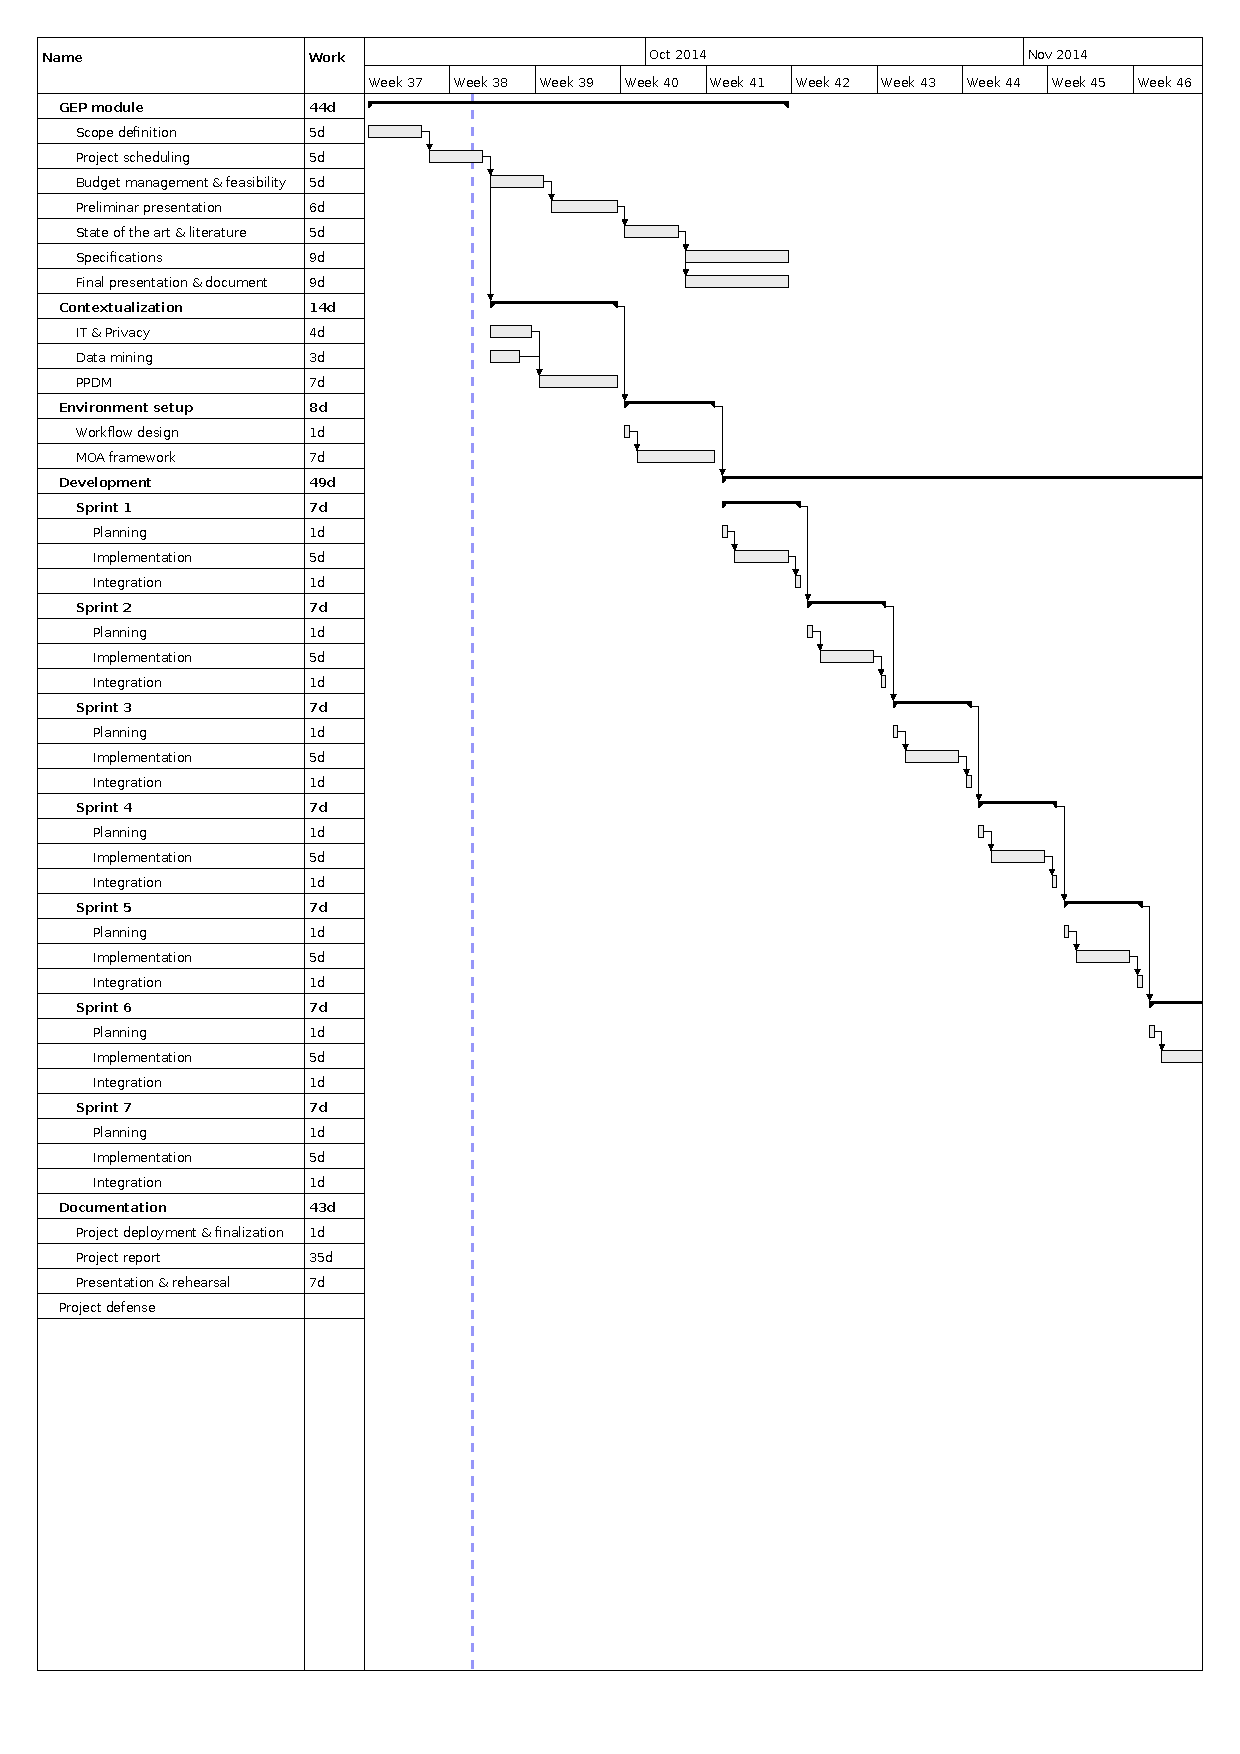
\includegraphics[trim={0 7.3cm 0 0},clip,page=1,width=1.2\linewidth]{figures/gantt-chart.pdf}
	}
	\caption{Initial project schedule Gantt chart (part 1).}
	\label{fig:gantt-1}
\end{figure}

\begin{figure}[hbtp]
	\makebox[\textwidth]{
		\includegraphics[trim={0 7.3cm 0 0},clip,page=2,width=1.2\linewidth]{figures/gantt-chart.pdf}
	}
	\caption{Initial project schedule Gantt chart (part 2).}
	\label{fig:gantt-2}
\end{figure}

\clearpage

\subsection{Schedule deviation}
\label{Management:Schedule:Final}

We will cover now the changes that have occurred in the schedule of the project and analyze its causes.

\subsubsection{Overall duration}

The original total duration has been extended from 5 months to 8 months, approximately. Thus, the final report and its defence is now scheduled to be in April, which is the next available lecture shift in the Faculty. We believe that this extended duration will allow us to fulfill all requirements defined in the scope of the project.

\subsubsection{Deviation analysis}

There are several possible reasons behind this schedule deviation:

\begin{itemize}
	\item The Project Management module lasted longer than expected, forcing the development phase of the project to begin later.
	\item During the definition of the project initial schedule, we expected to begin developing it while the Project Management module endured, which was, definitely, a planning error. Such tasks concurrency was not possible at that time.
	\item At the beginning of the development phase, we explored different technological alternatives, before deciding which approach was mostly suited to our needs, but this exploration delayed the actual development process for a couple of weeks.
	\item As was already stated in the Project Management report, some of the requested features have posed to be more complicated than was expected, consuming some more time than that assigned to them.
	\item For personal reasons, no work could be carried out during the Christmas vacations, which lasted two more weeks, furtherly delaying the project's development.
\end{itemize}

\subsubsection{Current detailed schedule}

Considering the previous analysis, a new Gantt chart has been built, with the new project's schedule, which is detailed in~\fref{fig:new-gantt-1} and~\fref{fig:new-gantt-2}.

\begin{figure}[hbtp]
	\makebox[\textwidth]{
		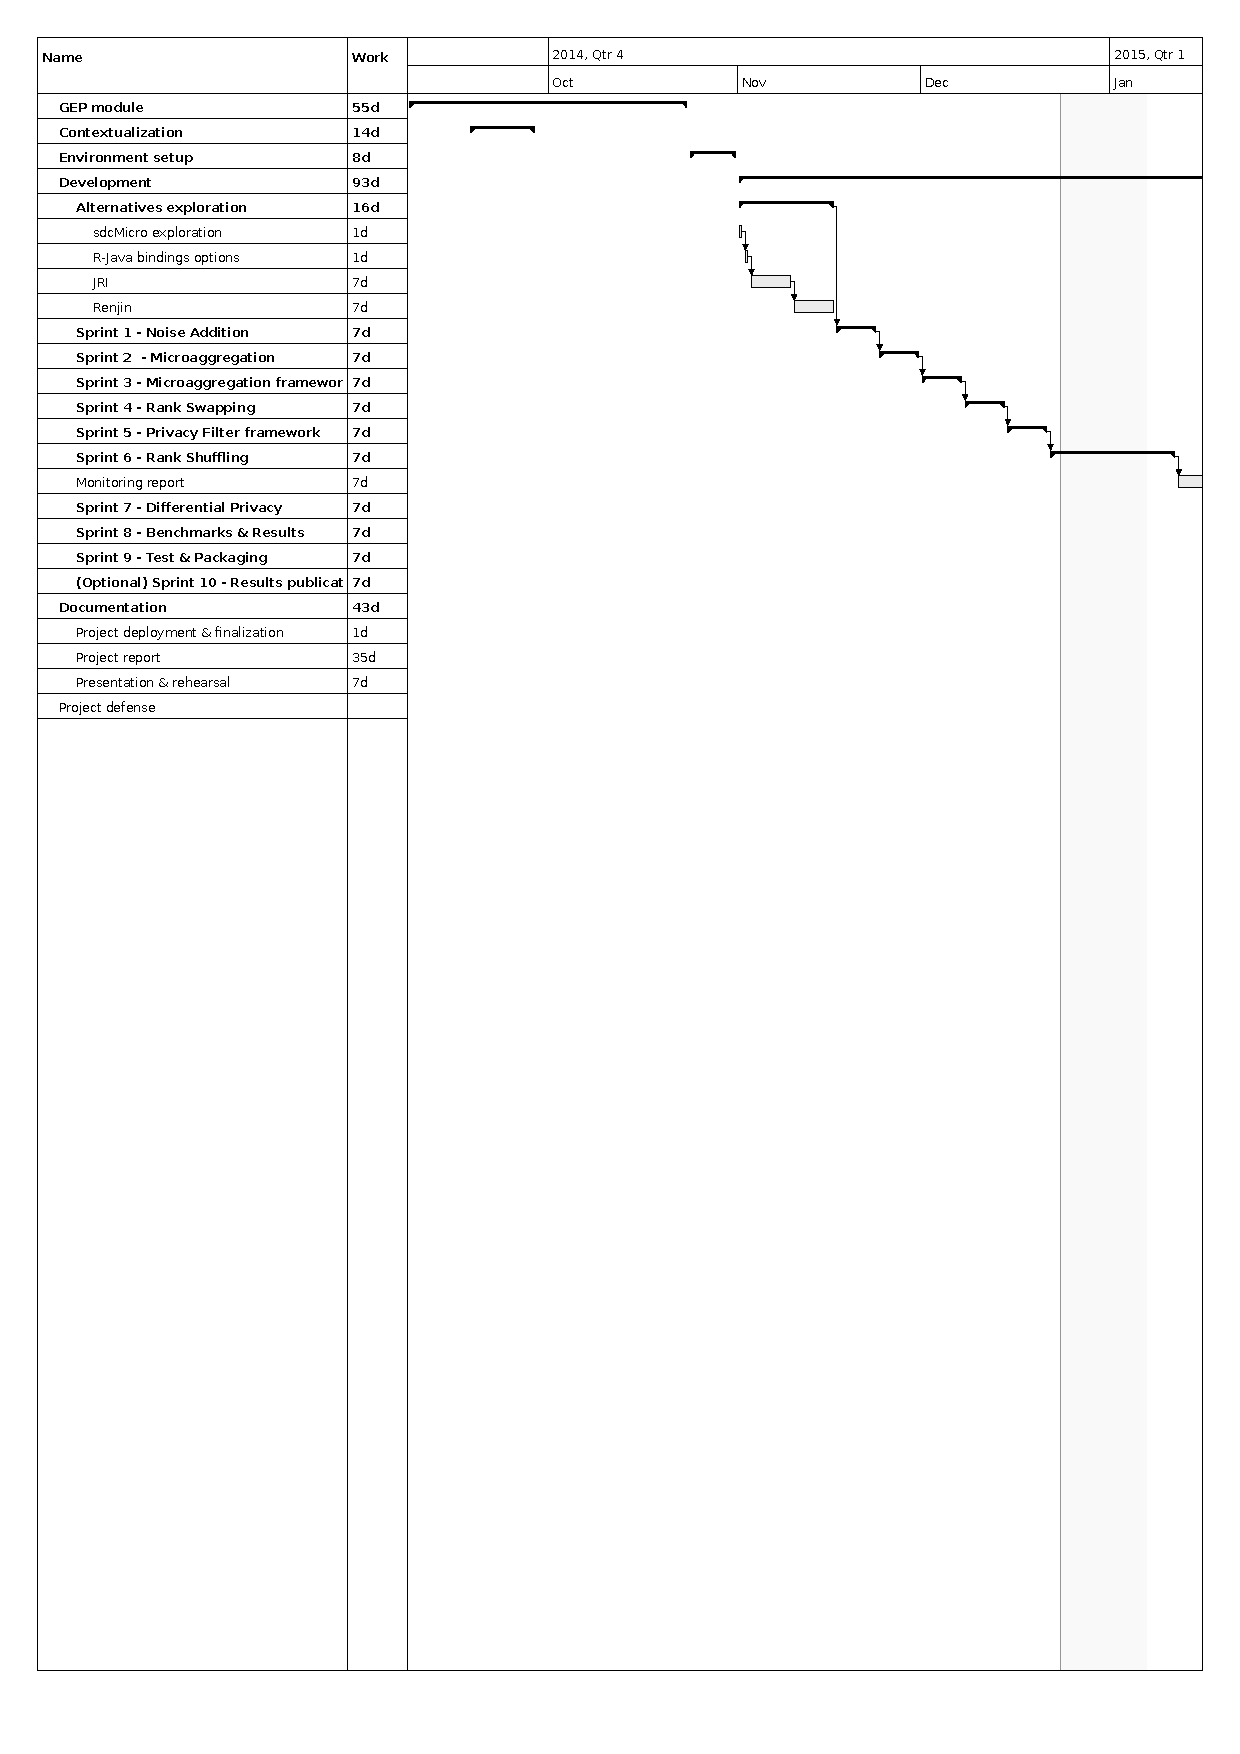
\includegraphics[angle=90,trim={0 17.5cm 0 0},clip,page=1]{figures/new-gantt-chart.pdf}
	}
	\caption{Final project schedule Gantt chart (part 1).}
	\label{fig:new-gantt-1}
\end{figure}

\begin{figure}[hbtp]
	\makebox[\textwidth]{
		\includegraphics[angle=90,trim={0 17.5cm 0 0},clip,page=2]{figures/new-gantt-chart.pdf}
	}
	\caption{Final project schedule Gantt chart (part 2).}
	\label{fig:new-gantt-2}
\end{figure}

\clearpage